% TFG - José Ángel Martín Baos. Escuela Superior de Informática. 2018
%%%% CHAPTER: Results %%%
\chapter{Results} % TODO
\label{chap:results}

\drop{I}{n} this chapter, the different results obtained during the execution of this \ac{BSc.} Thesis are presented. The working methodology presented in Chapter \ref{chap:methodology} is going to be used to carry out the work. In first place, the initial Sprint is presented, where the Scrum team will be set up, as well as the initial planning of the project. Subsequently, the different Sprints are presented, where the work planned in the initial Sprint will be carried out.




%%% Sprint 0
\section{Sprint 0: Initial planning}
In this first phase, Sprint 0, the main objective is to define the Scrum team, the user stories, the project plan, and the temporal and cost planning. Then, the draft (“Anteproyecto”) must be written. Once this Sprint has been completed, the project can start, as state in the temporal planning. The task associated to this initial Sprint can be shown in Table \ref{tab:Sprint0-Tasks}.

\begin{table}[hp]
	\centering
	{\small
		\begin{tabular}{|p{.7\textwidth}P{.1\textwidth}|}
	\hline
	\rowcolor{tabheadbg}
	\multicolumn{2}{|c|}{\textscale{.8}{\textbf{Sprint 0 tasks}}} \\
	\hline
	\hline
	\textscale{.8}{\textbf{Task}} 			& \textscale{.8}{\textbf{Estimate}} \\
	\hline
	Define the Scrum team					& 0,5h \\
	\hline
	Define the user stories					& 5h \\
	\hline
	Generate the project plan				& 2h \\
	\hline
	Generate the temporal planning			& 2h \\
	\hline
	Generate the cost planning				& 1h \\
	\hline
	Investigate about similar proposals								& 3h \\
	\hline
	Create a GitHub repository				& 0,5h \\
	\hline
	Write the draft (“Anteproyecto”)		& 21h \\
	\hline
	\textbf{Total} 							& 35h \\
	\hline

\end{tabular}
	}
	\caption{Sprint 0 tasks}
	\label{tab:Sprint0-Tasks}
\end{table}

\subsection{Scrum Team}
Following the scrum roles defined in Section \ref{5-ScrumTeam}, the Scrum team will have the following structure:
\begin{itemize}
	\item \textbf{Product Owner:} Ricardo García Ródenas
	\item \textbf{Scrum Master:} Luis Rodríguez Benítez
	\item \textbf{Development Team:} José Ángel Martín Baos
\end{itemize}

\subsection{Product Backlog}
\REDNOTE{... \& User Stories Table}
\begin{table}[hp]
	\centering
	{\small
		\begin{tabular}{ |P{.08\textwidth}p{.56\textwidth}P{.1\textwidth}P{.14\textwidth}|}
	\hline
	\rowcolor{tabheadbg}
	\multicolumn{4}{|c|}{\textscale{.8}{\textbf{User stories}}} \\
	\hline
	\textscale{.8}{\textbf{ID}}	& \textscale{.8}{\textbf{User history}}	& \textscale{.8}{\textbf{Priority}}	& \textscale{.8}{\textbf{Estimation (h)}} \\
	\hline
	1 	& Configure Raspberry Pi Architecture 										& High 		& 15 \\ 
	\hline
	2 	& Install PiCamera module in the Raspberry Pi								& High 		& 5 \\ 
	\hline	
	3 	& Develop an algorithm to calculate the vehicle flow		 				& High 		& 30 \\ 
	\hline
	4 	& Install environmental and gas sensors into Raspberry Pi					& High 		& 25 \\ 
	\hline
	5 	& Obtain and process data from the sensors									& High 		& 30 \\ 
	\hline
	6 	& Develop a comunication module using IBM IoT								& High 		& 15 \\ 
	\hline
	7 	& Receive sensor data from the Raspberry Pi and store it into a Database	& High 		& 12 \\ 
	\hline
	8 	& Integrate camera, sensors and comunication module into an unique program	& Medium	& 8 \\ 
	\hline
	9 	& Design a web page to monitor the data obtained by the Raspberry Pi devices	& High 		& 10 \\ 
	\hline
	10 	& Monitor in real time the data obtained by the devices and send an alert if the pollutant gases exceed a threshold																		& Medium 		& 20 \\ 
	\hline
	11 	& Display the historical data generated by the Raspberry Pi devices			& Low	& 20 \\ 
	\hline	

\end{tabular}
	}
	\caption{User stories}
	\label{tab:User-Stories}
\end{table}
	
The different user stories are presented its corresponding Sprints. Each user story is formed by the following fields:
\begin{itemize}
	\item \emlst{Sprint.} It indicates the Sprint number to which the user story belongs to.
	\item \emlst{Priority.} Priority given to the user story. It can take the values: low, medium and high.
	\item \emlst{Effort.} The estimated duration of the user story in hours. 
	\item \emlst{Name.} The label of the user story.
	\item \emlst{Description.} It is a brief definition of the user story.
	\item \emlst{Tasks.} It consists in a list of the different tasks that must be executed to complete the user story.
	\item \emlst{Tests.} It is a list of the different tests defined for the user story using \ac{TDD} as it is stated in Chapter \ref{chap:methodology}.
\end{itemize}

\subsection{Project plan}
\REDNOTE{Different sprints and its associated user stories and time estimation. \\
What is the total duration of the \ac{BSc.} Thesis?}
\begin{table}[hp]
	\centering
	{\small
		\begin{tabular}{|P{.08\textwidth}p{.56\textwidth}P{.15\textwidth}P{.08\textwidth}|}
	\hline
	\rowcolor{tabheadbg}
	\multicolumn{4}{|c|}{\textscale{.8}{\textbf{Sprints}}} \\
	\hline
	\hline
	\textscale{.8}{\textbf{Sprint}}			& \textscale{.8}{\textbf{Name}}	& \textscale{.8}{\textbf{User stories}}	& \textscale{.8}{\textbf{Estimate}} \\
	\hline
	0 	& Initial planning		 	& - 	& 35h \\ 
	\hline
	1 	& Development a basic algorithm to calculate the flow of vehicles		 		 	& 1, 2, 3 	& 50h \\ 
	\hline
	2 	& Design of an environmental parameters monitoring system		 	& \REDNOTE{...} 	& \REDNOTE{X}h \\ 
	\hline

\end{tabular}
	}
	\caption{Sprints}
	\label{tab:Sprints}
\end{table}

\subsection{Temporal planning}
\REDNOTE{Using the project plan, translate it to a graph (Remember the “Anteproyecto”)}

\REDNOTE{ Check the duration of all the task and sprints.} %TODO: Check the duration of all the task and sprints

\REDNOTE{The project start in September}

% Ganttproject


\subsection{Cost planning}
To manage the costs for the development of this project, two tables has been elaborated. Table \ref{tab:Hardware-Costs} indicates the costs related with the hardware resources that must be purchase in order to execute the project. Moreover, some development cost must be taken into account, which are indicated in Table \ref{tab:Development-Costs}. For the purpose of calculating the salary of the developer, the \ac{UCLM} retributions table of labor contracts for research projects on 2017 has been used. Therefore, it has been considered that the developer will have “Tercera-O-II” category, meaning that its annual cost will be of $23.598,83$\euro{}

\begin{table}[hp]
	\centering
	{\small
		\begin{tabular}{ |p{.5\textwidth}P{.1\textwidth}r|}
	\hline
	\rowcolor{tabheadbg}
	\multicolumn{3}{|c|}{\textscale{.8}{\textbf{Hardware costs}}} \\
	\hline
	\hline
	\textscale{.8}{\textbf{Item}}	& \textscale{.8}{\textbf{Quantity}}	& \textscale{.8}{\textbf{Cost}} \\
	\hline
	Raspberry Pi 3 					& 2 	& 49\euro{} \\ 
	\hline
	Pi NoIR Camera V2 				& 2 	& 28\euro{} \\ 
	\hline
	Memory card Samsung SDHC
	EVO 8gb Class 10+ 				& 2		& 8\euro{} \\ 
	\hline
	Power bank battery 				& 2 	& 29\euro{} \\ 
	\hline
	Camera Case		 				& 2 	& 14\euro{} \\ 
	\hline
	Raspberry Pi Sense HAT			& 2 	& 42\euro{} \\ 
	\hline
	Stacking Header 40 PIN 			& 2 	& 7\euro{} \\ 
	\hline
	MQ7 Gas Sensor		 			& 2 	& 2.5\euro{} \\ 
	\hline
	MQ2 Gas Sensor 					& 2 	& 3\euro{} \\ 
	\hline
	MCP3008 AD Conversor			& 2 	& 9\euro{} \\ 
	\hline
	Prototype shield  				& 1 	& 1.5\euro{} \\ 
	\hline
	Wires 							& 1 	& 7\euro{} \\ 
	\hline
	LM317 							& 2 	& 1.75\euro{} \\ 
	
	\Xhline{2\arrayrulewidth}
	\textbf{TOTAL:} &  		& \textbf{395\euro{}} \\ 
	\hline

\end{tabular}

	}
	\caption{Hardware costs}
	\label{tab:Hardware-Costs}
\end{table}

\begin{table}[hp]
	\centering
	{\small
		\begin{tabular}{ |p{.1\textwidth}P{.1\textwidth}r|}
	\hline
	\rowcolor{tabheadbg}
	\multicolumn{3}{|c|}{\textscale{.8}{\textbf{Development costs}}} \\
	\hline
	\hline
	\textscale{.8}{\textbf{Sprint}}	& \textscale{.8}{\textbf{Hours}}	& \textscale{.8}{\textbf{Cost}} \\
	\hline
	0			& 35h 			& \REDNOTE{X}\euro{} \\ 
	\hline
	\REDNOTE{XXX}	& \REDNOTE{X}h 		& \REDNOTE{X}\euro{} \\ 
	
	
	\Xhline{2\arrayrulewidth}
	\textbf{TOTAL:} & \textbf{\REDNOTE{X}h} 		& \textbf{\REDNOTE{X}\euro{}} \\ 
	\hline
	
	% Coste: Regla de 3:
	%    12 meses  ---- 23.598,83 euros
	%    X  meses  ---- Y euros
	% Jornada completa: 35 horas semanales

\end{tabular}
	}
	\caption{Development costs}
	\label{tab:Development-Costs}
\end{table}



%%% Sprint 1
\section{Sprint 1: Development a basic algorithm to calculate the traffic flows based on video data}
According to the project plan, in this sprint, a basic algorithm to calculate the vehicle flow must be developed. This involves executing the task associated to the user stories 1, 2 and 3. This iteration aims to obtain a basic algorithm to count the number of cars that cross a street in a certain amount of time so as to obtain the vehicle flow. \REDNOTE{Then in Sprint X, it will be improved.} To be able to count the number of cars using the PiCamera, \emword{motion vectors} are used. Therefore, a study about this concept has been done before implementing the algorithm. But first, it is necessary to configure the Raspberry Pi architecture and to install the PiCamera. 

\subsection{Sprint planning meeting}
During the planning meeting, the different user stories addressed in this sprint has been analysed. Consequently, they have been divided into several tasks and tests. The three user stories can be shown in Tables from \ref{tab:Sprint1-User-story-1} to \ref{tab:Sprint1-User-story-3}.

\UserStoryTable{1}{1}{High}{15}
{Configure Raspberry Pi Architecture}
{The \ac{OS} and all the components must be installed and configured.}
{	\item Install and configure Raspbian \ac{OS}
	\item Install the necessary libraries
}{	\item Check if the system works correctly using SSH connection
	\item Check if python works
}

\UserStoryTable{2}{1}{High}{5}
{Install PiCamera into Raspberry Pi}
{The PiCamera module must be working and some sample videos should be recorded in order to check the camera.}
{	\item Install the PiCamera module
	\item Develop a program to record videos
}{	\item Check if the camera is working correctly
}

\UserStoryTable{3}{1}{High}{30}
{Develop a basic algorithm to calculate the vehicle flow}
{Development of a basic algorithm that counts the number of cars that go across a street and determines their direction.}
{	\item Study the functionality of the motion vectors in H264/AVC
	\item Extract the motion vectors when recording a video with the PiCamera module using PiMotionAnalysis
	\item Read and process the data stored containing the motion vectors
	\item Develop a noise filter using moving averages
	\item Develop the basic algorithm to counts the cars
}{	\item Check the correctness of the motion vectors extracted
	\item Compare the data before and after applying the noise filter
	\item Assess the performance of the traffic-counting algorithm
}


\subsection{Results of the development of the tasks}
\textbf{Install and configure Raspbian \ac{OS} and the necessary libraries}

The first step consist of the Raspbian \ac{OS} installation, its configuration, and the installation of the necessary libraries. These steps are explained in the Appendix \ref{chap:installation_guide}. Once installed, the functionality of the system has been checked using a SSH connection from the development computer to the Raspberry, in order to ease the access to the System. 

\textbf{Install the PiCamera module and develop a program to record videos}

The next step is connecting the PiCamera module and configuring it as stated in Appendix \ref{chap:installation_guide}. Now, the device looks like in the Figure \ref{fig:6-Sistema_v1}. 

\begin{figure}[!h]
	\begin{center}
		\includegraphics[width=0.8\textwidth]{6-Sistema_v1.jpg}
		\caption{Device structure with PiCamera installed}
		\label{fig:6-Sistema_v1}
	\end{center}
\end{figure}

A configuration file has been implemented which contains some variables that are used by several modules of the device. Hence, these values are stored only once and can be changed easily. The whole file is shown and explained in Appendix \ref{chap:user_manual}. The parameters related with the camera are shown in Listing \ref{lst:6-camera-config}.

\lstinputlisting[language=Python, firstline=1, texcl, caption = {Part of \texttt{config.py} file containing the camera parameters}, label = lst:6-camera-config]{code/6-camera-config.py}

To assure the correct functionality of the camera, some videos are recorded. For that purpose and following the examples provided in PiCamera documentation \cite{PiCameraDoc}, a script has been developed. This script is shown in Listing \ref{lst:6-camera-video-recording}. This script must wait two seconds to ensure the camera is initialized correctly, then the camera starts recording during 60 seconds (as it is defined in \texttt{config.py}) and finally the video is saved in the file \texttt{my\_video.h264} in h264 video format.

\lstinputlisting[language=Python, firstline=1, texcl, caption = {Sample recording with PiCamera script}, label = lst:6-camera-video-recording]{code/6-camera-video-recording.py}


\textbf{Extract the motion vectors when recording a video with the PiCamera module using PiMotionAnalysis and PiMotionArray}

The result of the previous task allows recording videos using the PiCamera. This task deals with the need of extracting the motion data from the videos. To achieve this task, \texttt{PiMotionAnalysis} class from \texttt{picamera.array} is used. While recording is in progress, the incoming motion data is converted into a numpy array and an analysis method is called with the resulting array passed as argument. This class can be extended and the analysis method can be overridden. Therefore, in this method, the motion vectors can be used to detect movement in the video.

\BLUENOTE{Due to the fact that this class is used when the video is being recorded, it is used in the final implementation but first, in order to realize the different test, another class is used instead. The reason is that in this early steps of the work, it is more interesting to have the videos with the motion data stored into files and use them at any time. Hence, \texttt{PiMotionArray} class is used, which converts the incoming motion data into a numpy array also, but the conversion its made when the recording has finished. The class generates a 3-dimensional numpy array organized as (frames, rows, columns) where rows and columns are the number of the rows and columns of the macro-block \REDNOTE{(reference to the explanation of a macro-block)} in the frame. There is an extra column in the motion vector data that is not going to be used. Then, the data is stored into a file. 
}

\begin{figure}[!h]
	\begin{center}
		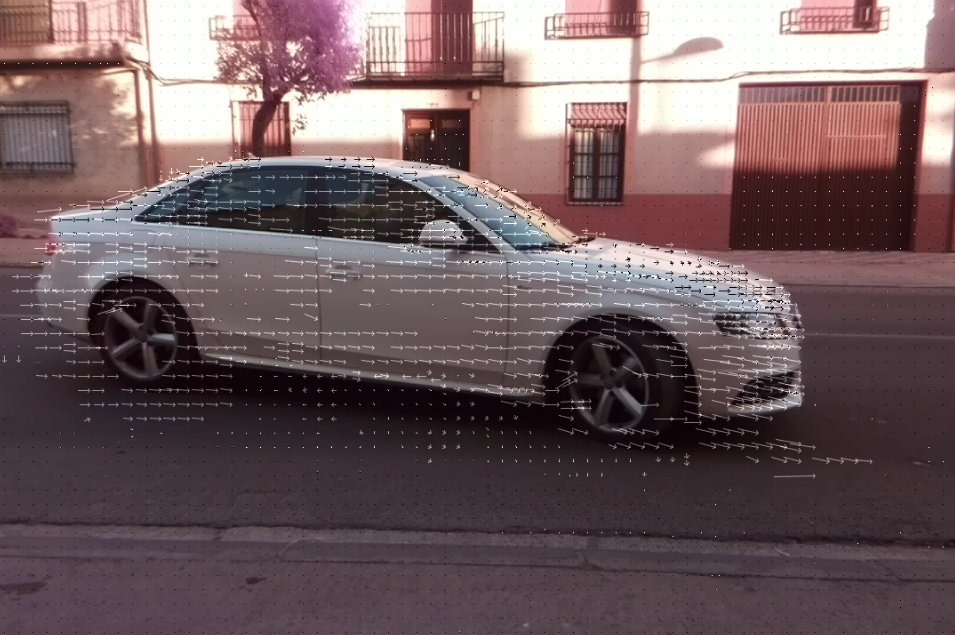
\includegraphics[width=0.8\textwidth]{6-Car_with_MV.png}
		\caption{Example of  the motion vectors taken by the Raspberry Pi}
		\label{fig:6-Car_with_MV}
	\end{center}
\end{figure}

The class used for recording the videos and the motion vectors used for developing the algorithm to count cars can be shown in Listing \ref{lst:6-Recorder-Sprint1}. Some parameters are given as arguments: \texttt{distance} and \texttt{angle}. They are used only for the filename so as to know afterwards the conditions of the camera when the video was recorded. In this class, the camera is configured according to the values stored in \texttt{config.py}. When the video has been recorded, it will be stored in a file with extension \texttt{.h264}, as well as the motion data, that will be stored in a file with the same name and extension \texttt{.data}. To finish with, the video will be also converted to \texttt{.mp4} to make easier its view in the development computer. 

\REDNOTE{IMPORTANT NOTE: Image resizer is not used. An other option is configure the camera resolution to 1920x1080 and use a resizer in the video to reduce the resolution given to the H.264 video coder.}

\lstinputlisting[language=Python, firstline=1, texcl, caption = {Class used to record a video and its corresponding motion data}, label = lst:6-Recorder-Sprint1]{code/6-Recorder-Sprint1.py}

\textbf{Develop a noise filter using moving averages}

There are some factors that can affect the number of motion vectors in a certain frame. Some of these factors can be the incorrect codification of that frame or a small object crossing the image (e.g., a person or a bug). Moreover, when H.264 video coding is used, there are several types of frame: I-frames, P-frames and B-frames \REDNOTE{(reference to their explanation)}. I-frames do not require other video frames to be decoded, therefore, they do not generate any motion vectors. Thus, the number of motion vectors in some frames is not going to be close to the reality, causing noise. To solve this problem, a smoothing technique is used. More concretely, simple moving averages calculation is applied.

A simple moving average \cite{Smi15} is a unweighted average of k prior values. Since a time series can be regarded as a sequence of values, $\{\overline {x_{t}}\}$, being $t=1,2,3,4,…n$, the moving average of these values can be computed. If we assume that $n$ is quite large, and we select an integer $k$ which is much smaller than $n$, we can compute the simple moving averages (of order k) as shown in Equation (\ref{eq:simple_moving_averages}).

\begin{equation} \label{eq:simple_moving_averages}
\overline { { x }_{ t } } =\frac { 1 }{ k } \sum _{ i=t-k+1 }^{ t }{ { x }_{ i } } ,\quad 2\le k\le n
\end{equation}

The result of applying the simple moving average over the data recorded previously can be shown in Figure \ref{fig:6-moving_averages}. Here, it can be appreciate how the graphic corresponding with the data before applying simple moving averages (black line) has some noise and sometimes it falls to 0. Additionally, it can be shown how the problem is decreased using this smoothing technique.

\begin{figure}[!h]
	\begin{center}
		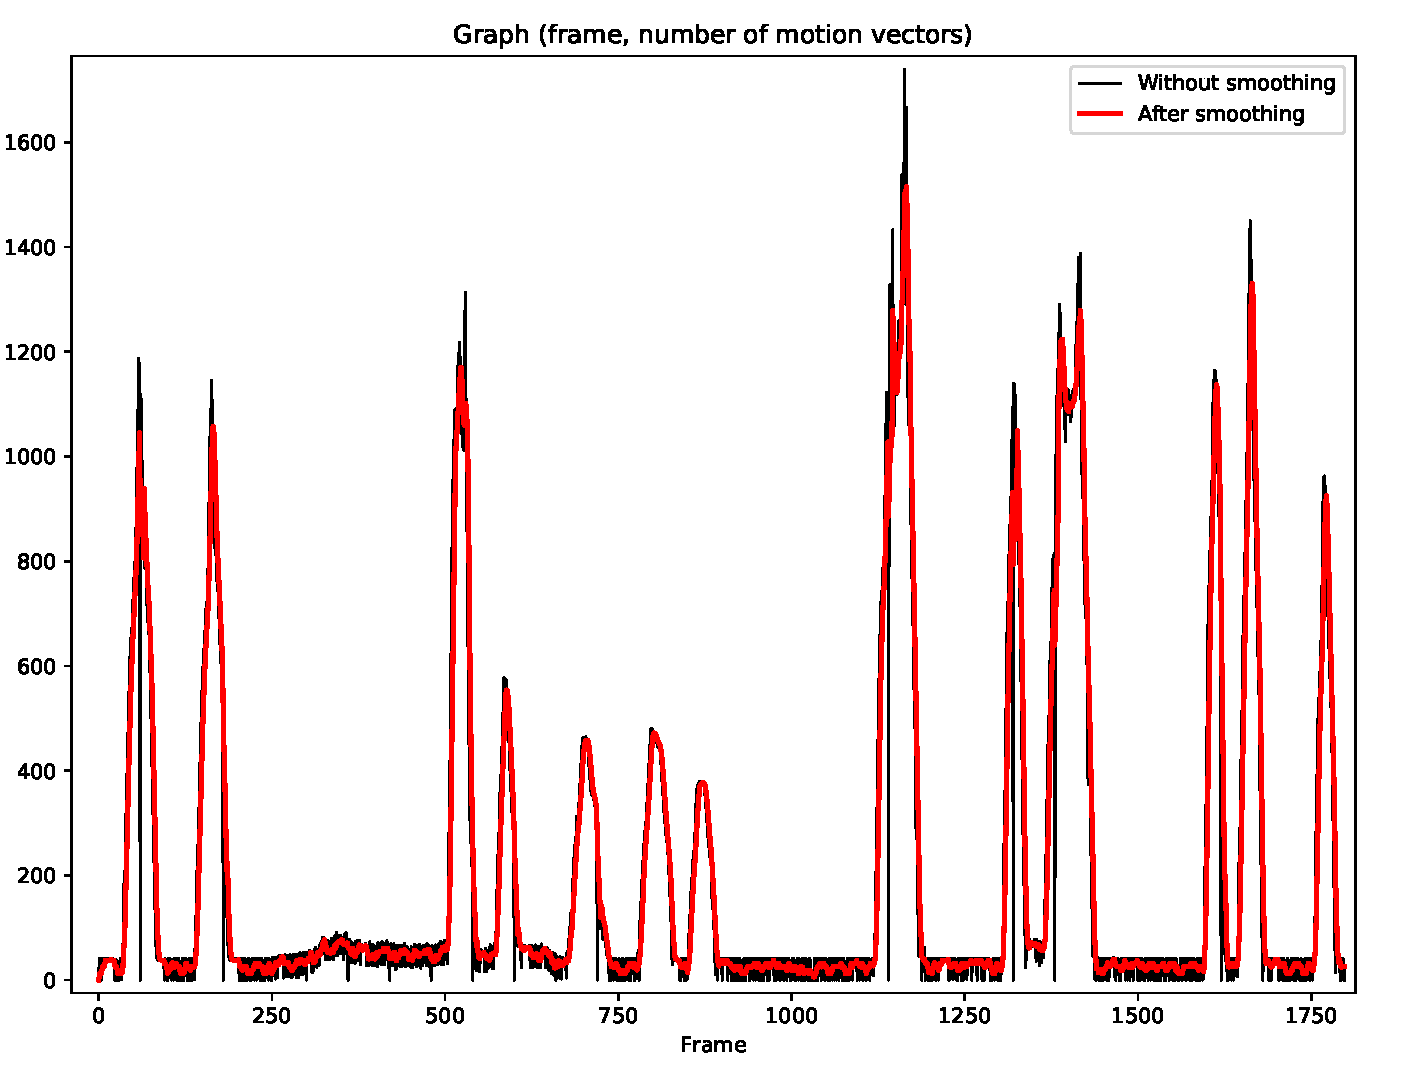
\includegraphics[width=1\textwidth]{6-moving_averages.pdf}
		\caption{Result of applying moving averages of order $n = 6$ to smooth the data}
		\label{fig:6-moving_averages}
	\end{center}
\end{figure}


\textbf{Develop the basic algorithm to counts the cars}

To count the cars that go across a street depending on its direction and using the motion data previously stored, an algorithm has been developed. Its pseudocode is shown in Algorithm \ref{alg:count_cars_V1}. This algorithm discriminates the cars direction (left or right). For each of the directions, the following algorithm is executed: 

For each frame, the number of motion vectors in that frame is compared with the number of vectors in the previous frame, increasing or decreasing a variable called \texttt{growth}. Once the number of frames exceed the \texttt{HEIGHT\_THRESHOLD} variable, if the \texttt{growth} variable is positive, the variable \texttt{n\_positive\_frames} is increased by one. If this last variable overtakes the \texttt{WIDTH\_THRESHOLD} variable, then we can consider that a new car has been detected. If the \texttt{growth} variable gets equal to \texttt{-GROWTH\_LIMIT}, then we consider that the car has already passed, and the variable \texttt{n\_positive\_frames} is restored to its initial value (zero).

An example of the execution fo the algorithm can be shown in Figure \ref{fig:6-Count_cars_graphic}, where the blue line represents the number of motion vectors with left direction for each frame, and the red line represents the same but for right direction. The black line, represent the \texttt{HEIGHT\_THRESHOLD} variable. Therefore, a car can be predicted if the number of frames in one direction overtakes the \texttt{HEIGHT\_THRESHOLD} variable during more than \texttt{WIDTH\_THRESHOLD} frames. And, it can be considered that the car has already cross if the number of frames has been decreasing $\texttt{GROWTH\_LIMIT} \times 2 $ frames, regardless if the number of motion vectors is under the \texttt{HEIGHT\_THRESHOLD} variable or not. Therefore, in Figure \ref{fig:6-Count_cars_graphic}, we can consider that two different cars have cross near the frame 1000, as the number of motion vectors has decreased during more than $\texttt{GROWTH\_LIMIT} \times 2 $ frames.

%\IncMargin{1em}
\begin{algorithm}
	\SetKwInOut{Input}{Input}\SetKwInOut{Output}{Output}
	\LinesNumbered
	\SetAlgoLined
	
	\Input{cols --> Number of colums with a macroblock in each frame\\
		rows --> Number of rows with a macroblock in each frame\\
		frames --> The number of frames in the video. \\
		motion\_data --> Array that contains a structure [x,y,SAD] for each frame} 
	\Output{n\_cars  --> Vector which contains the number of cars that has been counted crossing in left and right direction respectively.}
	
	n\_cars $\gets$ [0, 0]\;
	mv $\gets$ []\;
	smooth\_mv $\gets$ []\;
	car\_detected $\gets$ [False, False]\;
	growth $\gets$ [0, 0]\;
	n\_positive\_frames $\gets$ [0, 0]\;
	
	
	\For{frame $\gets$ 0 to frames}{
		%Add to the end of $mv$ vector a list with two elements. The first element consist in the number of motion vectors in that frame whose 'x' value is greather than the variable $GROUP\_SENSITIVITY$. The second element is the number of them whose 'x' value is lower than $-GROUP\_SENSITIVITY$.
		\tcc{Obtain number of motion vectors in each direction.}
		mv.append([ (motion\_data[frame]['x'] > GROUP\_SENSITIVITY).sum() ,
		(motion\_data[frame]['x'] < -GROUP\_SENSITIVITY).sum() ])\;
		
		\BlankLine
		\tcc{Apply moving averages to smooth the number of motion vectors}
		tmp\_left $\gets$ 0, tmp\_right $\gets$ 0\;
		\For{i $\gets$ 0 to SMOOT\_ORDER}{
			j $\gets$ frame - i\;
			\lIf{j < 0}{j $\gets$ 0}
			tmp\_left $\gets$ tmp\_left + mv[j][0] \;
			tmp\_right $\gets$ tmp\_right + mv[j][1]\;
		}
		smooth\_mv.append([tmp\_left / SMOOT\_ORDER, tmp\_right / SMOOT\_ORDER])\;
		
		\BlankLine
		\BlankLine
		\For{direction $\gets$ 0 to 2}{
			\uIf{smooth\_mv[frame-1][direction] < smooth\_mv[frame][direction]\\
				\hskip2em \textbf{and} growth[direction] < GROWTH\_LIMIT}{
				growth[direction] $\gets$ growth[direction] + 1\;
			}
			\ElseIf{smooth\_mv[frame-1][direction] < smooth\_mv[frame][direction]\\
				\hskip2em \textbf{and} growth[direction] > -GROWTH\_LIMIT}{
				growth[direction] $\gets$ growth[direction] - 1\;
			}
			
			\uIf{smooth\_mv[frame][direction] >= HEIGHT\_THRESHOLD \\
				\hskip2em \textbf{and} growth[direction] > 0}{
				n\_positive\_frames[direction] $\gets$ n\_positive\_frames[direction] + 1\;
				\If{n\_positive\_frames[direction] >= WIDTH\_THRESHOLD \\
					\hskip2em \textbf{and} car\_detected[direction] = False}{
					car\_detected[direction] $\gets$ True\;
					n\_cars[direction] $\gets$ n\_cars[direction] + 1\;
				}
				
			}
			\ElseIf{growth[direction] = -GROWTH\_LIMIT}{
				car\_detected[direction] $\gets$ False\;
				n\_positive\_frames[direction] $\gets$ 0\;
			}	
		}	
	}
	\caption{Count cars (First Version)}\label{alg:count_cars_V1}
\end{algorithm}\DecMargin{1em}

\begin{figure}[!h]
	\begin{center}
		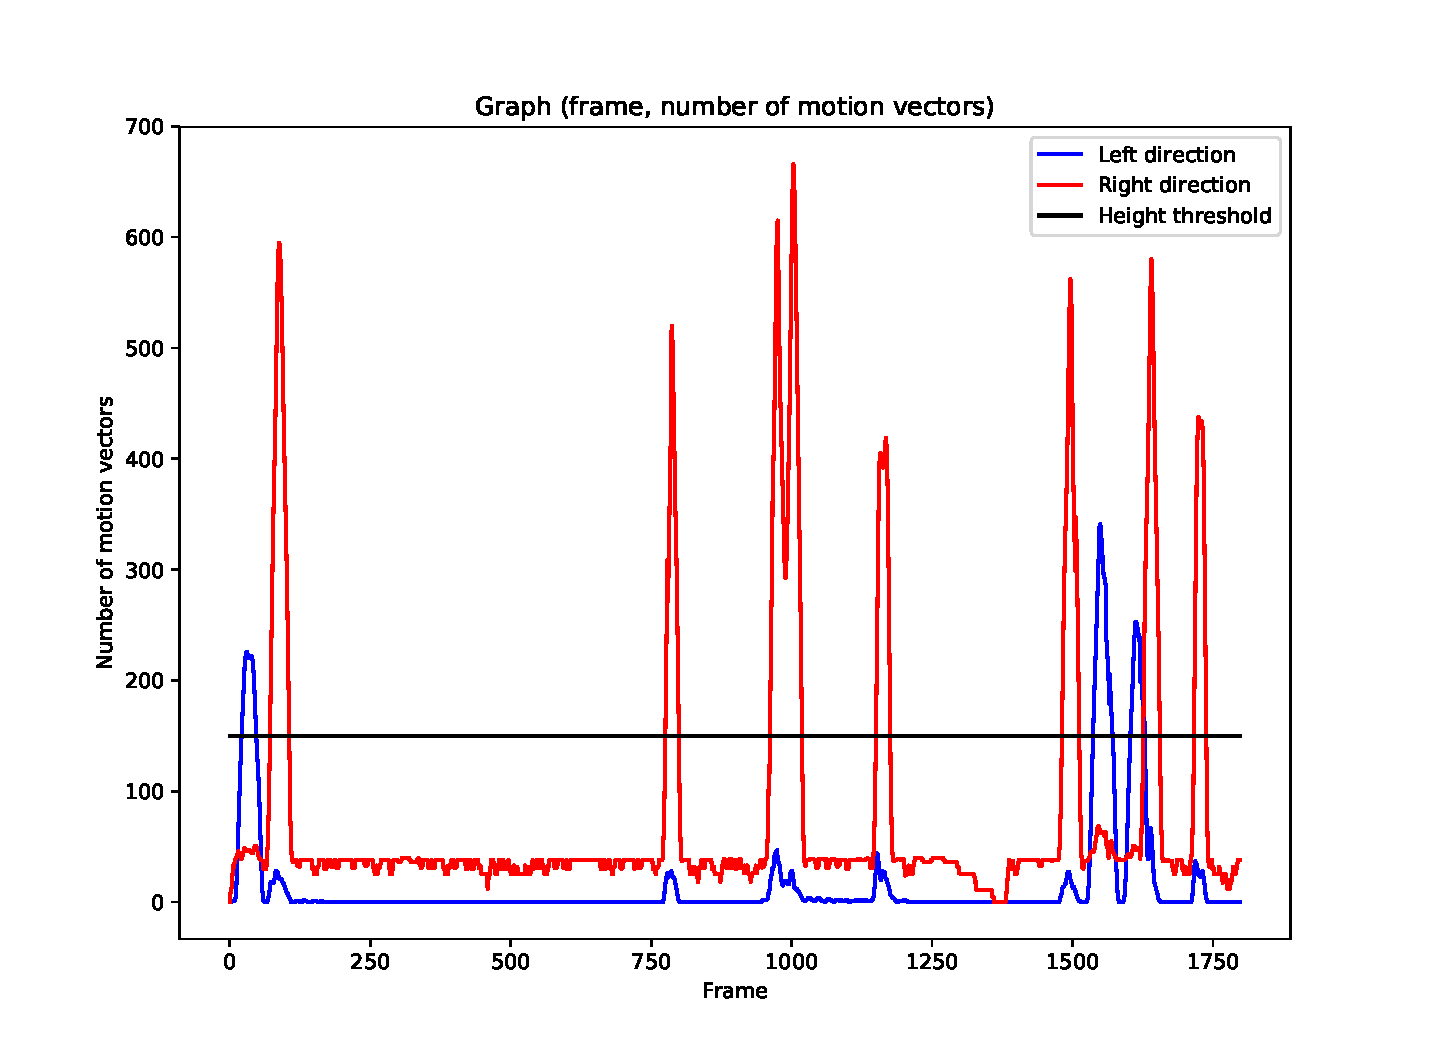
\includegraphics[width=1\textwidth]{6-Count_cars_graphic.pdf}
		\caption{Number of motion vectors in the test video 8}
		\label{fig:6-Count_cars_graphic}
	\end{center}
\end{figure}

Once the algorithm has been developed, it should be tested using the different videos recorded previously as it was stated in the list of test for the user story. The result of executing the algorithm over the different videos is shown in Table \ref{tab:Results_CountCars_V1}. After evaluating the results obtained, it is concluded that they are acceptable for the goal of this Sprint, therefore, a new Sprint can be started.

\begin{table}[hp]
	\centering
	{\small
		\begin{tabular}{ |P{.08\textwidth}P{.15\textwidth}P{.15\textwidth}P{.2\textwidth}P{.15\textwidth}|}
	\hline
	\rowcolor{tabheadbg}
	\multicolumn{5}{|c|}{\textscale{.8}{\textbf{Algorithm \ref{alg:count_cars_V1} results}}} \\
	\hline
	\hline
	\textscale{.8}{\textbf{Number}} & \textscale{.8}{\textbf{Quality}} & \textscale{.8}{\textbf{Camera angle}} & \textscale{.8}{\textbf{Distance to the road}} & \textscale{.8}{\textbf{Percentage of hits}} \\
	\hline
	1 	& 1080x720		 	&  center 		& 1m	& \textbf{100\%} \\ 
	\hline
	2 	& 1080x720		 	&  center 		& 1m	& \textbf{100\%} \\ 
	\hline
	3 	& 1080x720		 	&  center 		& 1m	& \textbf{90\%} \\ 
	\hline
	4 	& 1080x720		 	&  center 		& 2m	& \textbf{90.91\%} \\ 
	\hline
	5 	& 1080x720		 	&  center 		& 2m	& \textbf{100\%} \\ 
	\hline
	6 	& 1080x720		 	&  center 		& 2m	& \textbf{100\%} \\ 
	\hline
	7 	& 1080x720		 	&  center 		& 2m	& \textbf{94.74\%} \\ 
	\hline
	8 	& 1080x720		 	&  center 		& 3m	& \textbf{100\%} \\ 
	\hline
	9 	& 1080x720		 	&  center 		& 3m	& \textbf{90.91\%} \\ 
	\hline
	10 	& 1080x720		 	&  left 		& 1m	& \textbf{86.67\%} \\ 
	\hline
	11	& 1080x720		 	&  left 		& 1m	& \textbf{100\%} \\ 
	\hline
	12 	& 1080x720		 	&  left 		& 1m	& \textbf{100\%} \\ 
	\hline
	13 	& 1080x720		 	&  left 		& 2m	& \textbf{100\%} \\ 
	\hline
	14 	& 1080x720		 	&  left 		& 2m	& \textbf{55.56\%} \\ 
	\hline
	15 	& 1080x720		 	&  left 		& 2m	& \textbf{73.33\%} \\ 
	\hline
	16 	& 1080x720		 	&  left 		& 2m	& \textbf{88.89\%} \\ 
	\hline
	17 	& 1080x720		 	&  right 		& 1m	& \textbf{66.67\%} \\ 
	\hline
	18 	& 1080x720		 	&  right 		& 1m	& \textbf{78.57\%} \\ 
	\hline
	19 	& 1080x720		 	&  right 		& 1m	& \textbf{90\%} \\ 
	\hline
	20 	& 1080x720		 	&  right 		& 2m	& \textbf{83.33\%} \\ 
	\hline
	21 	& 1080x720		 	&  right 		& 2m	& \textbf{91.67\%} \\ 
	\hline
	22 	& 1080x720		 	&  right 		& 2m	& \textbf{88.89\%} \\ 
	\hline
	23 	& 1080x720		 	&  right 		& 2m	& \textbf{90\%} \\ 
	\hline
	\hline
	\multicolumn{3}{|c|}{\textscale{.8}{\textbf{Total number of tests: }} 23} & \multicolumn{2}{|c|}{\textscale{.8}{\textbf{Global percentage of hits: }} \textbf{89.57\%}} \\
	\hline
	
\end{tabular}
	}
	\caption{Results of the Algorithm \ref{alg:count_cars_V1} over the first test dataset}
	\label{tab:Results_CountCars_V1}
\end{table}


\REDNOTE{Task: Create a module that use the counting algorithm to obtain the vehicle flow in real time (using PiMotionAnalysis) in this Sprint or in another one.}

\REDNOTE{Do we need to comment the different Scrum events?}



%%% Sprint 2
\section{Sprint 2: Design of an environmental parameters monitoring system}
\REDNOTE{...}
% Product Backlog refinement

\subsection{Sprint planning meeting}
\REDNOTE{...}

\UserStoryTable{4}{2}{High}{x}
{Name of the user story}
{A description of the user story}
{	\item Task A
	\item Task B
	\item Task C
}{	\item Test A
	\item Test B
}

%Table \ref{tab:Sprint2-User-story-4}

\subsection{Results of the development of the tasks}
\textbf{task something ...}

\REDNOTE{...}

\cite{LM317,ADC,MQ7,MQ2,SenseHAT,ConfMQX}




%%% Sprint 3
\section{Sprint 3: ....}
\REDNOTE{Task: Create a module that use the counting algorithm to obtain the vehicle flow in real time (using PiMotionAnalysis) in this Sprint or in another one.}
\REDNOTE{...}
% Product Backlog refinement

\subsection{Sprint planning meeting}
\REDNOTE{...}

%\UserStoryTable{4}{3}{High}{x}
%{Name of the user story}
%{A description of the user story}
%{	\item Task A
%	\item Task B
%	\item Task C
%}{	\item Test A
%	\item Test B
%}

%Table \ref{tab:Sprint2-User-story-4}

\subsection{Results of the development of the tasks}
\textbf{task something ...}

\REDNOTE{...}

\subsection{Daily Scrum}
\REDNOTE{...}

\subsection{Sprint review}
\REDNOTE{...}

\subsection{Sprint retrospective}
\REDNOTE{...}
